%\makeevenhead{plain}{\thepage}{\textit{Animal Breeding Plans}}{}
%\makeoddhead{plain}{}{The Origin and Domestication of Farm Animals}{\thepage}

\chapter{The Origin and Domestication of Farm Animals}
\label{cha:origin-and-domestication}
\index{Domestication|(}
\index{Evolution|(}

The story of the origin and domestication of farm animals, although interesting, has little practical
usefulness to the animal breeder who is seeking to better his flocks and herds today. Only living
animals can be used for breeding; and if those have the inheritance the breeder wants and can produce
fertile offspring, it makes little difference how they came by that inheritance or what their ancestors
were. Knowledge of how closely two races of animals are related may be of some help in forecasting the
outcome of crosses between them; but such predictions, based on degree of relationship, will have many
exceptions. Knowledge of the origin of farm animals, therefore, is useful to the practical breeder only
in the same way that ancient history may be useful in training modern people for citizenship. The 
details matter not at all, but here and there the history may show with dispassionate clearness some 
general principle of human conduct which will repeat itself in present situations. Also, it may give 
the student a perspective which will be useful in making decisions concerning contemporary affairs. The 
present chapter, then, is a compilation of facts which may be helpful in forming a historical 
perspective from which to view the present general problems of animal breeding. The reader seeking 
only immediately useful information is advised to omit it or merely glance at it.

\textit{Domestication} of the important farm animals was accomplished long before the beginning of written
history, but long after man had become a toolmaker and tool-user of considerable skill. In terms of human
culture it seems to have happened mostly very late in the Paleolithic (Old Stone Age) or early in the
Neolithic (New Stone Age), although this varied with different peoples in different parts of the world.

The \textit{origin of the species} of animals which were domesticated extends back into vastly greater
reaches of time and is only a special aspect of the story of evolution. Figure~\ref{fig:Lush_Figure_1} is intended to show
graphically the contrasts in the enormously long time involved in evolution, the comparatively short
time which has elapsed since domestication first took place, and the tiny fraction of time since definite
and continuous written history began.

The following comments concerning geologic and cultural time are centered around man and other mammals,
since those are the central figures in the story of domestication. There are hundreds of thousands of
species in the animal kingdom; but with a few exceptions, such as honeybees and silkworms, all the
domesticated animals are included in a few species of mammals and birds. It is an interesting but perhaps
an idle speculation to wonder why so few species were domesticated. Did the mental characteristics of the
others make domestication impossible? Or did those which were domesticated have among them nearly all the
characteristics which man found useful to him? Why did not man domesticate any of the many species of animals
which hibernate through the winter? Those would have had some practical advantages in regions where feed is abundant from spring to
fall, but scarce or buried during the winter. Are there perhaps still unrealized possibilities which can be had
by domesticating species which are still wild or semi-wild?

\begin{figure}[htbp]
    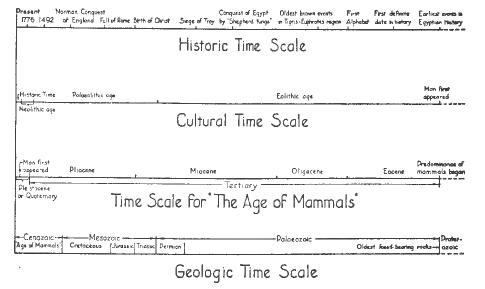
\includegraphics[width=\textwidth]{Figure_1.png}
    \caption{The comparative lengths of historic, cultural, and geologic time. Each line represents on an expanded scale the small segment at the extreme left end of the line just below it. If the geologic scale were drawn with the same number of years per inch as the historic one, it would need to be more than 20 miles long!}
    \label{fig:Lush_Figure_1}
\end{figure}

\index{Feral}Domestication implies several things, no one of which alone is sufficient to define it completely. It usually
means tameness, but individual wild animals may be tamed (as trained seals or performing bears are) without our
being willing to call them domesticated, and ranch-raised but nevertheless domesticated cattle or horses may be
very wild individuals. Domestication implies bringing the animal's growth and reproduction at least partly under
man's control, but we call pigeons and cats domesticated, even though their breeding habits and mating choices
usually are not controlled by man. Domestication implies that man converts the animal's products or services to
his own advantage or purposes, but he does this also with many wild animals, such as the fur-bearing ones. Some
of the domesticated ones, such as canaries, many breeds of dogs, and most \index{``Pet and fancy stock''}``pet and fancy stock'' serve him only
in an aesthetic way. As the word implies, domestic animals usually are kept in or near man's own dwelling places,
but usually we do not consider as domesticated the mice and rats which live in man's barns or even in his own
houses, while we do consider range-raised cattle and sheep as domestic animals although they may never have seen
a human habitation. Some of the domestic animals are dependent on man's care for their very existence, at least
in many regions. But horses, dogs, and even cattle, have at times run wild and reproduced for several generations
without any control or care by man. Strictly speaking such animals are called ``feral'' rather than truly wild.
Domestication has in most cases produced rather large changes in behavior. Some of these are conditioned by the
environmental circumstances under which the domestic animal is reared but many of them are hereditary and
presumably have been caused during the process of domestication by selection for those individuals or families
which were the gentlest, the most cooperative with man, the best trail-runners (in the case of some breeds of
dogs), etc.

In the laboratory animals, or the animals used in fish farming and in fur farming, we may perhaps be witnessing
the slow process of domestication. Some of them, like the guinea pig or the white rat, have almost as good a
claim to be called domesticated as do swine or reindeer or ducks. Others, such as mink and silver foxes, have
advanced little beyond the stage of wild animals being kept in cages as in a menagerie.

\section*{GEOLOGIC TIME}

The Cenozoic Era (the Age of Mammals) began some 50 to 75 million years ago, although the expression of geologic
time in years, particularly in the more remote periods, is very uncertain. The first mammals had come from a
reptile group called Cotylosaurs through a premammal group called Cynodonts some time in the enormous interval
between the beginning of the Permian and the end of the Triassic, but they did not become the dominant form of
animal life until the Cenozoic, being overshadowed earlier by the reptile forms. The Cenozoic is divided into
five periods, which, as far as the mammals are concerned, are chiefly noted as follows:

\textsc{Eocene}. The archaic or generalized mammals were replaced by 
modern types.

\textsc{Oligocene}. The mammals differentiated into many of the orders and families known today. An anthropoid
(Propliopithecus) is known from early in this period.

\textsc{Miocene}. This period saw the greatest variety and abundance of mammalian forms. It was a period of
extensive grasslands and restricted forest areas over much of the earth. Corresponding to that, there was a
widespread expansion and development of the grazing forms of mammals at the expense of the browsing forms. It
is probable that man's line of descent had already diverged from that of the other anthropoids by the middle
of the Miocene.

\textsc{Pliocene}. Most modern genera and even some modern species of mammals already were present at the
beginning of the Pliocene. Man's definitely human ancestors appeared during this period at a time date of
something like 600,000 to 1,000,000 years ago.

\textsc{Pleistocene}. There was periodic glaciation and with it the extinction of many of the great mammals,
such as the mammoth, the mastodon, the woolly rhinoceros, the saber-toothed tiger, and many others. Man
learned the use of tools and fire and began to domesticate animals for his own use. The period ends with the
retreat of the last great glaciation about 30,000 years ago.

\textsc{Recent} (The Age of Man). Civilization began. The historical aspects of what is known about man and his
surroundings constitute the subject matter of archaeology, and archaeology in turn gives way to history when
the written records become adequate enough to give a connected account of man's activities.
\index{Evolution|)}

\section*{CULTURAL OR ARCHAEOLOGICAL TIME}

Archaeological time is measured in stages of human culture. It does not correspond perfectly to chronological
time, since human culture did not advance contemporaneously in all parts of the world. The major subdivisions
of cultural time are as follows:

\textsc{Pre-Human Period} (the Eolithic or dawn period). This period begins with the time when man's ancestors
can first be called definitely human, something like a million years ago, and extends roughly to the coming of
pre-Neanderthal man in Europe about 200,000 years ago. The use of tools was advanced but little beyond picking
up and using such stones or clubs as happened to be handy. Probably fire was not used.

\textsc{Paleolithic Period} (the Old Stone Age). This period was marked by the use of stone and bone implements
which slowly increased in complexity and usefulness. The use of fire was learned at least by the time of
Neanderthal man. No agriculture was practiced; and there were no domesticated animals, except perhaps the dog.
The Paleolithic culture in Europe slowly developed to Neolithic culture around 25,000 years ago. What was
practically Paleolithic culture still prevailed among the aborigines of Australia and Tasmania and the Bushmen
of South Africa when the first white explorers came in contact with them.

\textsc{Neolithic Period} (the New Stone Age). This period was marked by the use of ground and polished bone and
stone weapons and tools. Neolithic man made pottery and crude textiles and basketwork. He practiced agriculture
in a crude way. He had domesticated animals of nearly all the species we have today, whereas Paleolithic man had
few or none. Neolithic man lived in huts or even in wooden houses as, for example, the Swiss Lake Dwellings. The
art of metal-working was still unknown or was practiced only on soft metals used for ornaments. The American
Indians were in a rather advanced stage of Neolithic culture when the first white explorers found them. The
cultures of the Aztecs, Mayas, and Peruvian Indians already were more advanced in many ways than the late
Neolithic cultures of Europe. They were working copper, silver, and gold, but those metals were too soft to
make useful tools. The Neolithic culture of the American Indian was behind that of Europe in the use of domestic
animals.

As long ago as 4500--4000 B.C., the city of Tepe Gawra in the Tigris valley included in its culture such things
as gold and lapis lazuli beads, temples, landscape painting, and the firing of painted pottery, although the
inhabitants had not learned to smelt copper. The earliest bit of copper known is an ornamental pin made in Egypt
perhaps as long ago as 5000 B.C. The Egyptians were working the copper mines in the Sinai peninsula regularly for
ornaments by 3500 B.C. and were using copper tools by 3000 B.C.

\textsc{Bronze Age}. The use of bronze began in Assyria by 3000 B.C. and spread west and northwest like a slow
wave. It had certainly reached the Danube basin by 2000 B.C. and perhaps Britain almost that early. Apparently
there was no bronze age in Africa, except in Egypt and on the northern coast. The other African races went
directly from the stone age into the iron age. In the bronze age in Europe, village life and complex social
customs had already developed far.

\textsc{Iron Age}. Bits of iron have been found in the Great Pyramid at Gizeh (about 2900 B.C.), but apparently
these were only rare curiosities. General use of iron for tools or weapons was begun by the Hittites in Asia
Minor about 1300 B.C. and iron supplanted bronze as the commonest metal for weapons among the Assyrians by 1000
B.C. Then its use spread rapidly.

History and archaeology are intertwined in the long period which we describe loosely as the ``dawn of history.''
The earliest definite date in history is 4236 B.C., when the Egyptian calendar began; but fragments of Egyptian
history are known from nearly 5000 B.C. Some time between 5000 and 4000 B.C. the Egyptians began to use ox-drawn
plows, and by 3500 B.C. they had an alphabet. The beginnings of history were not contemporary in different parts
of the world. For example, the definite history of Britain begins about the time of the Roman conquest; and that
of the Scandinavian countries begins about five or six hundred years later. Little is known of South Africa or
Australia before 1500 A.D. On the other hand, the history of Greece goes back some 2000 years farther than that
of Britain; Cretan history is known from nearly 3000 B.C., and a few events among the Sumerians near the Persian
Gulf can be dated at about 3500 B.C.

\section*{DATE OF DOMESTICATION OF FARM ANIMALS}

All the farm animals were domesticated long before historic times. The evidence about when and how that happened
is incomplete and consists of such things as the bones and tools found buried in the trash heaps around ancient
camp sites or caves, the drawings or carvings on the walls of caves or on ornaments. Rich sources of evidence are
the tools, weapons, utensils, and images which so many peoples placed in the graves with their dead.

Often such evidence is fragmentary and may be interpreted with equal plausibility in several different ways. Even
where evidence admits only one interpretation, the dates derived from it are necessarily minimum dates. For example,
the evidence leaves no doubt that domesticated horses were widely used in the region of the Tigris and Euphrates
rivers as long ago as 2000 B.C. and probably the first of them were brought into that region as long ago as 3000
B.C. Even if the earliest date of domesticated horses in this ``two-river land'' were established with absolute
certainty, it still remains possible that horses may have been domesticated and used a thousand years earlier at
some other place as yet unexcavated. Doubtless the thoroughly excavated sites of ancient human camps and cities
are only a small fraction of the total number which exist and may be discovered in the future.

One who reads the technical evidence and discussions can scarcely avoid the feeling that they give an unduly large
emphasis to details of the shape of horns and skull. This is natural since these parts of the animal are best
preserved and best known. It is partly justified because these parts are little affected by ordinary variations
in nutrition or other environmental influences. Yet one who surveys the considerable variability in skull and
horn shape within comparatively pure breeds today, and who considers the known cases where a single gene
substitution can cause large differences in these characteristics, must feel uneasy about placing much faith in
genealogies which rest largely on similarities or differences in the size and shape of horns or skulls. Such
genealogies are especially questionable when they are based on only a few specimens, perhaps widely separated
in time.

It is uncertain that Paleolithic man in Europe actually domesticated any animal, although he may have had the dog.
The Paleolithic aborigines who settled in Australia took the dog with them, but no other modern animal. Paleolithic
man in Europe used the horse extensively for food, but it is probable that he hunted it as game and had not really
domesticated it.

Neolithic man in Europe appears to have had nearly all of our modern domestic animals except the cat and poultry
and those animals which were found only in America or in the tropics. Some students of the evidence claim that
even in early Neolithic times the bones of the domesticated ox, swine, and sheep were already distinctly different
from their wild contemporaries. There is even considerable speculation that the domesticated races of the early
Neolithic in Europe were brought from the Caspian region or from Asia Minor in an already domesticated condition
by peoples who migrated into Europe then. A considerable amount of care was certainly given to farm animals by the
Lake Dwellers and by the men of the bronze age. It is not certain that the horse was really a domesticated animal
in Europe before the end of the Neolithic, although the men of the bronze age certainly were riding horses.

The rock-carvings from ancient Egypt and from the pre-Babylonian peoples of Sumer and Akkad, which are among the
oldest of what may be called written records, show the goat, sheep, ox, ass, pig, dog, and cat. Caring for these
animals was already a well-established part of agricultural practice, even at that remote day.

\section*{PLACE OF DOMESTICATION}

Domestication took place in the Old World except in the case of the llama, alpaca, guinea pig, and turkey, which
are native to the Americas. In the Old World, domestication seems to have taken place largely in central or
western Asia, although the evidence points to some domestication in Egypt and in Europe itself. Chickens and
elephants were domesticated in India, and at least one center of domestication for swine was in China. Domestication
may have taken place independently in several regions. This seems certainly to have happened in the case of
swine and sheep and may have happened with other animals. Much of the world, especially central Asia, is still
incompletely explored from this point of view. There were no modern mammals (except the dog and man) in Australia.
Africa south of the Sahara desert had a fauna rich in mammalian species, but none of the domesticated animals,
except the South African ostrich and the African elephant, came from there. Upper Egypt or Ethiopia was one of
the centers of domesti.cation for the ass.

\section*{SPECIES DOMESTICATED}
\index{Species|(}

For many animals it is still disputed whether they descended from a single wild species (monophyletic origin) or
from two or more wild species perhaps domesticated in different regions or at different times and later interbred
(polyphyletic origin). The main reasons for this dispute are, of course, the scantiness of the evidence and the
different biological views which the writers hold. In many cases domestication was completed so long ago that the
original wild ancestor has become extinct, or it may still be living but the domesticated form has been changed so
much that we are not now certain which contemporary wild species was the ancestor.

Polyphyletic theories are not as widely held now as formerly. The idea of organic evolution was not generally
accepted even by naturalists until well into the last half of the nineteenth century. Many of the naturalists
who wrote on the origin of domesticated animals still had in their minds traces of the old Linnean idea of the
fixity of the species. Often they had an exaggerated idea of the supposed uniformity of wild species. With this
mental background a polyphyletic origin seemed to them the only possible way to explain the tremendous diversity
of domesticated forms --- for example, the tremendous contrasts between breeds of dogs or of sheep. Modern studies
of large samples from wild populations have shown that those populations are not as uniform as many of the older
naturalists believed. Some of these modern studies have shown that enough of this variability in wild populations
is hereditary that selection, directed toward diverse goals, and other breeding practices, such as inbreeding,
could in a few generations produce distinctly contrasting races from a single wild population if man were to
control its breeding as he does that of his domesticated animals. Hence it no longer seems necessary to invoke
a polyphyletic origin as an explanation for observed diversity. The possibility remains, however, that some
domesticated animals may really have had in their ancestry crosses of distinct races or even species which were
still genetically similar enough for their crosses to be fertile. This seems to have happened in the case of
swine and sheep, although there is plenty of room for difference in opinion as to whether the races domesticated
were ever different enough and discontinuous enough to justify calling them different species. The whole question
of proper taxonomic terms for domesticated animals is in a chaotic condition. Many taxonomists hold (with
Linnaeus) that variations among races of domesticated animals are largely man-made and therefore outside the
scheme of nature which is the concern of taxonomy.
\index{Species|)}

\section*{METHOD OF DOMESTICATION}

Literally nothing is known about how domestication was first accomplished. It is only speculation to guess that
hunters first brought home a few young as pets or captured cripples from time to time and thus learned how to
care for animals. At least one Egyptian rock-picture shows hunters building a fence across the mouth of a little
steep-walled valley into which they have driven some wild animals. Wild elephants are captured in India today by
carefully planned drives. Tame elephants are then used to help chain the wild ones and to teach them to work.
Hunger is the most generally effective method of taming the most unruly among the wild ones. But it is more
difficult to tame the African elephant, even by these same methods. This suggests that temperamental aptitude
was an important element in the success or failure of early attempts at domestication.

\section*{DETAILS ABOUT DIFFERENT KINDS OF DOMESTIC ANIMALS}

\textsc{Swine}. The European wild boar (\textit{Sus scrofa}) still lives in some of the forests of Europe. It
crosses freely with domestic swine, and the offspring are fertile. Doubtless it was domesticated somewhere around
the Baltic sea in Neolithic times. A swine race or species (generally known as \textit{S. vittatus}, although
some divide it into two groups and give the name \textit{S. cristatus} to one) native to the middle and eastern
Asian mainland from western India around to central China, and found also in nearby island lands like Japan,
Formosa, Sumatra, Java and Borneo, was separately domesticated in China, perhaps as long ago as 3000 B.C. At
least one more center of domestication in Neolithic times was south or southeast of the Alps, where some of the
Mediterranean local wild races were domesticated. \textit{S. scrofa} grades into \textit{S. vittatus} by a
gradual but continuous series of local races to such an extent that modern writers (such as Kelm, 1938) are
inclined to consider them all as one highly variable species --- a \textit{``Formenkreis''}; i.e., a chain or
circle of local groups or races, each differing only a little from the ones next to it but considerably from
those farther away.

Nomadic peoples could not move swine with them easily. They generally regarded with contempt the farmers and
settled valley-dwellers who did keep swine. This may have been the origin of the Hebrew and Moslem dislike of
swine, which was later fortified by religious precept. Because nomads could do so little spreading of swine
and because wild swine by themselves do not usually migrate far, there has been in swine more than in most
species a differentiation into local races which vary from one place to another. It may be more accurate to
speak of the practice of domestication spreading from tribe to neighboring tribe rather than to speak of an
actual spread of one or of a few domesticated forms of swine.

Some of the early navigators report finding native swine on some of the islands in the southern Pacific; but
the Polynesians who settled those islands were expert navigators who had come from the general Malaysian region
only a few centuries earlier, and probably they brought swine with them. The peccaries, which belong to a
different genus, are the nearest American relatives of swine. They had not been tamed by the Indians nor, from
their behavior in captivity, does it seem likely that they can be domesticated. The breeds of swine common in
the United States probably get most of their ancestry from the European wild swine, but there may have been a
considerable amount from the Mediterranean races, and there is clear historical evidence of the introduction
of at least a little blood from Chinese swine.

\textsc{Cattle}. The family Bovidae are the most specialized of the hollow-horned ruminants. They are connected
with the other ruminants by way of antelope-like ancestors from which they diverged in the Pliocene or Miocene.
Living forms of the Bovidae include the true buffalo, the bison, musk-ox, banteng, gaur, gayal, yak, and zebu,
besides what we commonly call cattle. The musk-ox is intermediate in some respects between oxen and sheep or
goats. The musk-ox has not been domesticated, although Stefansson reports that it is well suited for
domestication. The Asiatic buffalo was in Syria in Neolithic times, but may not have been domesticated until
near Christian times. It is an important dairy and work animal of India and lands farther east and is used a
little as far west as Bulgaria. It existed in the Atlas region of northwestern Africa even after Neolithic
times. The African buffalo has never been domesticated. The banteng, gaur, and gayal are all restricted to
south-eastern Asia and the nearby islands. The banteng is the common work ox of Java, Bali, and Borneo. It is
often crossed with common cattle, but the crosses thus produced are fertile. The gayal may be only the
domesticated form of the gaur. The European bison, or wisent, and the American bison have never been really
domesticated, despite a few sporadic attempts to do so. The American bison can be crossed with common cattle,
but there is much mortality and sterility among the crossbreds. The yak is the bovine species best adapted
to cold mountain lands. It is native to the highlands of Asia north of the Himalayas and, although an
important domestic animal there, has not found practical use outside that region. Nothing very certain is
known about its date of domestication. The yak can be crossed with common cattle and with zebus and with
bison, but there seems to be some sterility among the males from such crosses.\footnote{Deakin, Alan, Muir,
G. W., and Smith, A. G. 1935. \textit{Hybridization of Domestic Cattle, Bison, and Yak}. Publication 479,
Department of Agriculture, Dominion of Canada.}

There are in the whole world between six and seven hundred million cattle which are commonly grouped under
the one species name of \textit{Bos taurus}, although some prefer to give a separate species name,
\textit{B. indicus}, to the zebu group. In the Balkans, Asia Minor, central Asia, Korea, Formosa, and in
eastern and southern Africa , there is a wide variety of forms intermediate in many respects to the extreme
zebu types and the cattle of western Europe. The more extreme types have been separate in their ancestry
for thousands of years. Carvings from the Indus valley region show bulls with extreme zebu characteristics
from as long ago as the third millenium B.C. The cattle of the United States are of purely European origin,
except some in the region bordering the Gulf of Mexico, which have considerable zebu ancestry. Concerning
the ancestry of European cattle, the most commonly mentioned species or subspecies are: (1) \textit{B. taurus}
brachyceros (or longifrons), which was in Europe as a domesticated animal early in the Neolithic and presumably
was domesticated somewhere north of the Alps or in northwestern Asia; (2) \textit{B. taurus} primigenius, the
urus or aurochs, known in Caesar's time as the wild ox of Europe\footnote{Keller says the last wild aurochs cow
in Poland was killed in 1627.} but domesticated long before (perhaps early in the Neolithic), probably south
of the Alps or in the Balkans or in Asia Minor; and (3) \textit{B. namadicus}, which was contemporary with man
in India in the early Pleistocene. Other names, common in the early writing but not seen so often now, include
\textit{B. taurus frontosus}, the Swiss spotted cattle; \textit{B. taurus brachycephalus}, the short-headed
cattle such as the Dexter, Eringer and Zillertaler breeds; and \textit{B. taurus akeratos}, the hornless
cattle of northern Europe.

\textsc{Horses}. Horses were plentiful in Europe in Paleolithic times. That they were used for food is attested
by the cracked and dismembered bones, mostly of young horses, around old camp sites like that of Solutre near
Lyons. They were probably not domesticated at that time but were hunted for food. The horse is primarily adapted
to open grassland country and apparently became rare in Europe during Neolithic times with the increasing forest
growth. Formerly it was thought that a distinct type of forest horse remained in western Europe through the
Neolithic and was the principal ancestor of the heavy or ``cold-blooded'' draft breeds. More recent studies
(Antonius, 1936) indicate that the heavy horse was developed between 1000 and 1200 A.D. in or near Friesland out
of the existing domesticated horses of Tarpan origin. Prawochenski, however, disagrees with this interpretation.
Horse bones are rare in Neolithic deposits, but bronze age deposits include bridle bits and other accoutrements
thus proving its domestication by that time.

Probably all domesticated horses of Europe and western Asia descend from the tarpan which still existed wild in
eastern Europe in the region from East Prussia southward as recently as 1700 A.D. and perhaps in the 1800's.
Some writers distinguish between a ``forest tarpan'' in the more westerly region and a ``steppe tarpan'' farther
south and east, but others think (Antonius, 1936) there was no real distinction. In eastern Asia the wild horse
of Przewalskii was reported about 50 years ago and perhaps still exists in the Mongolian desert region. It may
have been domesticated separately there. The use of the horse had reached China before historic times, but that
is of uncertain date.

The horse first appears definitely in western history before 2500 B.C. when the Neolithic Indo-Europeans from
the Caspian basin brought it into Anatolia and later to Babylonia. Presumably the Indo-Europeans from west of
the Caspian took domesticated horses westward with them north of the Black Sea at more or less the same time.
Certainly horses were in Spain and northwest Africa before any could have reached there from Egypt. The horse
first reached Egypt about 1800 B.C. when the Shepherd Kings conquered Egypt from the northeast.

The \textit{evolution} of the horse is especially well known compared with that of other mammals and is used
as a classic illustration in many books on evolution and zoology. Most of this evolution took place in the
Americas, but horses later became extinct there after some of them had migrated to Asia. There were no horses
in the Americas when the white men came. Why they died out is one of the unexplained mysteries of evolution.
Conditions were favorable for them at the time of the discovery of America by white men, as is shown by the way
the horses which escaped from the early settlers or explorers multiplied. The wild horses of the present western
ranges are descendants of these escaped horses and are often used to illustrate the difference between ``feral''
animals and truly wild ones whose ancestors never have been domesticated.

The early use of horses was for human transport and for pulling chariots in time of war. Their use for pulling
loads and for tilling the soil is a comparatively modern development.

\textsc{Asses}. The ass was in common use in Egypt and Babylonia many centuries before the horse was introduced
into those lands. Probably it was originally domesticated in Egypt or on the east coast of Africa or in southern
Arabia or around the Persian gulf. Its nearest wild relatives are found in Africa and in Asia Minor. The main
(perhaps the only) ancestor is thought to have been the Nubian wild ass, although another variety of wild ass in
Somaliland may have contributed something.

It is generally stated that the other Equidae, such as the zebra, the kiang, and the onager, have not been
domesticated. However, Antonius concludes that the ancient Sumerians had domesticated the onager and used it
extensively, even for crossing with horses to produce mules\index{Mules}. Also it is stated\footnote{The Horse Lover. 7:9.
1943.} that Burchell's zebras were formerly used on stage lines in the Transvaal.

\textsc{Sheep and Goats}. The subfamily Ovinae are all highland or mountain dwellers. Perhaps because of this
and the resulting isolation they are mightily given to breaking up into many species, subspecies, varieties,
and local races. There is no single trait which distinguishes all goats from all sheep, although there are some
things which are characteristic of most sheep and few goats or vice versa. Besides the true sheep and the true
goats, there are, according to Antonius, the following groups of Ovinae: (1) The Hemitragus group of primitive
or short-horned goats with four teats. Three living species are found in the mountains of India and southern
Arabia. (2) The ibexes or steinbocks, which resemble the true goats rather closely and are fertile with them
but have contributed nothing to their ancestry. They are all mountain dwellers, and Antonius lists seven species
in the mountains from the Himalayas to the Pyrenees and another from the mountains of southern Abyssinia. (3)
The burrhel or blue sheep of Tibet. (4) The maned sheep or aoudad, now restricted to the Atlas mountains but
extending as far east as Egypt even in historic times. (5) The argali group, which are rather sheep-like and
include an enormous number of local races besides the argali itself and Marco Polo's sheep. The argali group
probably did not contribute anything to the ancestry of domesticated sheep, unless perhaps something to the
fat-rumped races. This is disputed by some investigators (Gromova, 1936) who believe the argali group was
important in the ancestry of domesticated sheep. (6) The thick-horned sheep, of which there are an enormous
number of local races extending from the northern Himalayas northeastward over Kamchatka and Alaska to
California. The Big Horn Sheep of the Rocky Mountain region is an example. Probably this group played no
part in the ancestry of domestic sheep. There have been a few accounts of crosses between domestic sheep
and Big Horn Sheep in western United States.\footnote{Jour. Wildlife Management 9:82-83. 1945.}

Domesticated goats are believed to descend mostly from \textit{Capra prisca}, which is known from Pleistocene
fossils from Greece northward, or from \textit{C. aegagrus}, the Bezoar goat or Psaang, which still exists
through the mountainous regions of Asia Minor and Persia and in the past has extended from Sind to as far west
as Crete. Also mentioned among the true goats are \textit{C. dorcas} (which some think only a form of
\textit{C. prisca}) from the Jura mountains, and \textit{C. falconeri}, which is extraordinarily given to
the development of distinct local races and lives in the region around Afghanistan. Some of the tame Egyptian
goats resemble \textit{C. falconeri} rather closely, but it is not certain that they descend from it in any
part. Nothing is known about the place of domestication of the goat, nor about the date of domestication,
except that it must have been very remote.

Domestic sheep are thought to descend mainly from the mouflon, \textit{Ovis musimon}, which is still found
wild in Sardinia and Corsica and interbreeds freely with domesticated sheep, and from \textit{O. vignei},
the urial, which is found from Turkestan to Asia Minor. Some writers think that a part of the ancestry of domesticated 
sheep came from \textit{O. orientalis}, the mouflon of Asia Minor and Armenia, or from \textit{0. arkal}, which is
found east of the Caspian Sea. There is more confusion and disagreement about the ancestry and classification of sheep 
than of any other farm animal.

Domestication of the sheep took place so long ago that taxonomic names have even been given to the forms found in 
deposits from various stages of human culture. Thus, there is talk of a ``turbary sheep, 
\textit{Ovis aries palustris}'' and of a ``copper-age sheep, \textit{Ovis aries studeri}.'' Early Neolithic man in Europe 
certainly had domesticated sheep with him, but where or when he got them can only be conjectured from what is known
about their geographical distribution. There is an enormous variety of breeds and races of domesticated sheep. The 
classifications proposed for convenience in referring to these are generally based on the nature of their wool and the 
length and fatness of their tails. Antonius classifies them for that purpose as follows:
\begin{enumerate}
	\item[1.] Long-tailed sheep
	\begin{enumerate}
		\item[A.] The wool sheep of Europe. These include all the breeds which are prominent in the United States.
		\item[B.] Hairy sheep originally prevalent all over Africa. The black-headed Persian sheep of South Africa is an example.
	\end{enumerate}
	\item[2.] Fat-tailed sheep, usually with a long tail, fat at the upper end but slender at the tip. Karakuls are an example.
	\item[3.] Short-tailed sheep, such as the Heidschnucke of Germany and other marsh or moorland sheep of northern Europe. 
	\item[4.] Fat-rumped sheep, which were originally native to high Asia east of where the fat-tailed sheep developed.
\end{enumerate}

\textsc{Dog}. Zoologically the dog is essentially the same as the common wolf of the northern hemisphere.\footnote{Crosses
between dogs and wolves are frequent (Jour. of Genetics 43:359--414. 1941).} The dog was the only 
domesticated animal found in both the New and the Old Worlds. The polyphyletic origin of the dog, involving the jackal
as well as the wolf, was once widely believed, but that belief has almost disappeared now. The dog may very well have 
been the first animal domesticated. Chaldean and Egyptian monuments show several distinct breeds in existence four or 
five thousand years ago. The Incas in Peru had bulldogs as well as their ordinary breed (Hilzheimer, 1936).

\textsc{Cat}. The Egyptians domesticated the African wild cat. Thence it was probably introduced to Italy by Phoenician 
traders some centuries before the Christian era. A European wild cat and perhaps also a Chinese wild cat may have 
contributed to the ancestry of modern domestic cats. 

\textsc{Camel}. The single-humped camel, \textit{Camelus dromedaritts}, was domesticated probably in Arabia or 
northeastern Africa, perhaps near the very beginning of Egyptian civilization or perhaps not until near 1000 B.C.
The two-humped camel, \textit{C. bactrianus}, was domesticated in Asia somewhere between Iran and the Gobi desert.
It had reached Syria at least by 1000 B.C. and perhaps a thousand years earlier. It is now the common camel in China
and the regions just northwest, although the other occurs also. 

The llama and alpaca are the only living American representatives of the camel family, although that family went
through most of its evolution in North America. They were domesticated by the ancient Peruvians from the wild
guanaco, \textit{Lama huanachus}, long before the Spanish conquest. The wild vicuna, \textit{L. vicugna}, is a close
relative. In the Incan agriculture the alpaca occupied somewhat the place of the sheep in ours, but the llama was used 
extensively as a beast of burden, as well as for its meat and wool. Llamas sometimes are used for dairy purposes, too. 

\textsc{Reindeer}. \textit{Rangifer tarandus} is the Scandinavian wild form which was domesticated by the Lapps
and later introduced to Alaska and arctic Canada. \textit{R. caribou}, the caribou of Canada, has not been
domesticated. One report has it that reindeer were domesticated in the Yenisei River basin about the time of Christ. 

\textsc{Elephants}. Elephants were domesticated at least as long ago as in ancient Carthage. Presumably they were
used in India much earlier. Alexander used them in his battle with Darius in 331
B.C.\footnote{See Armandi's ``Histoire militair e des elephants.'' Paris. 1843.} in Mesopotamia. 

\textsc{Chickens}. Chickens came from southeastern Asia and are generally believed to have descended from
\textit{Gallus bankiva}, the jungle fowl of India. It is not certain that more than one species was involved. 
Domesticated chickens were kept in China at least as early as 1400 B.C., and from India had arrived in Babylon by 600
B.C., in Greece by 500 B.C., and in Rome well before the Christian era. The actual introductions may have been
centuries earlier. 

\textsc{Geese}. These came from the grey laggose, \textit{Anser anser}, and perhaps also the Chinese goose,
\textit{Cygnopsis cygnoides}. The date is uncertain, but geese were kept by the ancient Romans several centuries
before the Christian era, as witness the legend about the cackling of the geese which on one occasion saved Rome
from invaders. There may have been several independent domestications.

\textsc{Ducks}. Probably these all come from the mallard duck, \textit{Anas boschas}, although there are many other 
species of wild ducks. Ducks probably were not domesticated before Roman times. 

\textsc{Guinea}. The guinea comes from the Guinea coast of western Africa. The wild species is
\textit{Numida meleagris}. The guinea was known to the Romans as a domestic fowl but later ceased to be kept in
Europe and was reintroduced by the Portugese in the sixteenth century.
 
\textsc{Peacock}.\textit{Pavo cristatus} is found in India and Ceylon. \textit{P. muticus} is found in Burma and
Java. Either or both may have contributed to the origin of domestic races. The peacock was a relatively late arrival
in European agriculture. It was first domesticated in Persia, or at least first knowledge of it came to Europe from 
Persia. 

\textsc{Turkey}. The peoples of ancient Mexico and Peru had domesticated the turkey long before the discovery of
America by white men. The wild Mexican turkey, \textit{Meleagris mexicana}, is thought to have furnished 
most of the ancestry, but \textit{M. gallopavo} from the Atlantic coast of the United States and \textit{M. ocellata} 
from Central America are sometimes mentioned in that connection. 

\textsc{Fur-Bearing Animals}. Such animals as the \textit{fox}, \textit{mink}, \textit{marten}, \textit{ferret},
\textit{skunk}, \textit{muskrat}, etc., are extensively reared in captivity but probably should not yet be called
truly domesticated. They may represent stages in domestication through which our farm animals passed far back in
Neolithic times.

\textsc{Laboratory Animals}. Among the laboratory animals, the \textit{guinea pig} probably should be called
domesticated. South American Indians were breeding it in captivity for food before the white man came. The
\textit{white rat} is an albinotic strain  of the common Norway rat, \textit{Mus norvegicus}. Probably the albino rat
was domesticated before the beginning of the nineteenth century. An albino rat colony in England in 1822 is reported. 
Fancy races of \textit{mice} were known in ancient Troy perhaps as long ago as 1200 B.C. and probably in China as far
back as 1100 B.C., since a Chinese dictionary of that date had a special word for the spotted mouse. Domestic
\textit{rabbits} are descended from the European rabbit, \textit{Oryctolagus cuniculus}. It was probably domesticated
in the Spanish peninsula or southern France, perhaps as early as 1000 A.D. 

\textsc{Bees}. Honeybees are mentioned frequently in the Old Testament and in early Roman writings on agriculture.
They were brought to America from Europe. Bumblebees were already in America when the first white explorers came.

\textsc{Silkworm Culture} developed in China, possibly longer ago than 2000 B.C. It did not spread to other countries
until the Christian era. 

\section*{REFERENCES}
Encyclopedias, especially the \textit{New Brittanica} and the \textit{Americana} and Volume 3 of Bailey's
\textit{Cyclopedia of American Agriculture}, furnish a good starting point for general information. Consult several
in order to note the disagreement as to fact and the confusion about specific classification.

The \textit{National Geographic Magazine} occasionally has an article on some domestic animal with pictures and 
descriptions of many of the living breeds or races. Some of the recent ones are as follows: 
\\
\begin{hangparas}{0.25in}{1}%
November, 1923. The story of the horse. W. H. Carter. 44:455-66.

December, 1925. The Taurine World. A. H. Sanders. 48:591-710.

April, 1927. The races of domestic fowl. M.A. Juli. 51:379-452.

March, 1930. Fowls of forest and stream tamed by man. M.A. Juli. 57:327-71.

April, 1935. Man's winged ally, the busy honeybee. James I. Hambleton. 67:401-28.
\end{hangparas}

Many of the original articles which treat of domestication in detail are in the German language, being written by 
Germans, Austrians, or Swiss. Among the more recent of these, should be mentioned:

\begin{hangparas}{0.5in}{1}%
(Various authors). 1936. Neue Forschungen in Tierzucht und Abstammungslehre. Bern: Verbandsdruckerei 
A.G. (contains the articles by Gromova and by Hilzheimer).

Antonius, Otto. 1922. Grundz\"{u}ge einer Stammesgeschichte der Haustiere. 336 pp. Jena: G. Fisher.

---. 1936. Zur Abstammung des Hauspferdes. Zeit f. Z\"{u}cht. B. 34:359-98.

Kelm, Hans. 1938. Das postembryonale Schadelentwicklung des Wild- und Berkshire-Schweins. Zeit. f. Anal. u. Entwicklungsgeschichte 108:499-559.

Klatt, B. 1928. Entstehung des Haustiere. Berlin: Gehr\"{u}der Borntraeger. 
\end{hangparas}

In the English language the following original articles or books treat of domestication in some detail:

\begin{hangparas}{0.5in}{1}%
Allen, R. L. 1847. Domestic animals. 227 pp. New York: Orange Judd \& Company.

Amschler, Wolfgang. 1935. The oldest pedigree chart. The Jour. of Heredity, 26:233-38.

Brown, Edward. 1906. Races of domestic poultry. 234 pp. London: Edward Arnold.

Ewart, J. Cossar. 1926. The origin of cattle. Proc. of the Scottish Cattle Breeding Conference for 1925, pp. 1-16.

Holmes-Pegler, H. S. 1929. The book of the goat. 255 pp. London: The Bazaar, Exchange and Mart.

Jennings, Robert. 1864. Sheep, swine, and poultry. Philadelphia: John E. Potter \& Company.

Lydekker, Richard. 1912. The horse and its relatives. 286 pp. London: G. Allen \& Company.

---. 1912. The ox and its kindred. 271 pp. London: Methuen \& Company.

---. 1913. The sheep and its cousins. 315 pp. New York: E. P. Dutton \& Company.

Morse, E. W. 1910. The ancestry of domesticated cattle. pp. 187-239 in the Twenty-seventh Annual Report of the Bureau of Animal Industry, United States Department of Agriculture.

Ridgeway, William. 1905. The origin and influence of the Thoroughbred horse. 538 pp. Cambridge University Press.

Shaler, N. S. 1895. Domesticated animals. 267 pp. New York: Charles Scribner's Sons.

Among French books, the following is unique enough to warrant special mention:

Chollet, et al. (since 1903) Les Animaux. 550 pp. Paris: Bong et Cie.
\end{hangparas}

Among the general references, dealing briefly with man's cultural stages while he was domesticating the 
animals or with evolutionary aspects of the subject, may be mentioned:

\begin{hangparas}{0.5in}{1}%
Breasted, J. H. 1938. The conquest of civilization. 669 pp. New York: Harper Brothers.

Matthews, W. D., and Chubb , S. H. 1921. Evolution of the horse. No. 36 of the Guide Leaflet Series, American Museum of 
Natural History, New York City.

Newman, H. H., et al. 1927. The nature of the world and of man. (pp. 332-80 for the story of man and civilization.) 
University of Chicago Press.

Sumner, F. B. 1932. Genetic, distributional and evolutionary studies of the sub-species of deer mice (Peromyscus). Bibliographia Genetica, 9:1-106.
\end{hangparas}